\atstartofhistorysection
\section[Un peu d’histoire : mesurer le degré de chaleur]{Un peu d’histoire :\onlyamphibook{\\} mesurer le degré de chaleur}
\label{ch_histoire_degre_chaleur_depondt}

\begin{center}\textit{Par Philippe Depondt\\ \begin{small}Université Pierre et Marie Curie, Paris\end{small}}\end{center}

	Pour Aristote, au \textsc{iv}\ieme siècle avant J.C. en Grèce, le feu était l'un des quatre constituants de la matière avec l'eau, l'air et la terre. L'idée de mesurer quelque chose, le feu ou autre, c'est-à-dire de donner une valeur numérique à une grandeur, lui était parfaitement étrangère car sa physique était essentiellement non-mathématique~\cite{koyre1966} : ses théories étaient basées sur des observations \emph{qualitatives}. La synthèse des idées d'Aristote avec le christianisme a été faite au \textsc{xii}\ieme siècle par Thomas d'Aquin et ces idées ont été très largement dominantes dans le monde savant en Europe jusqu'au début du \textsc{xvii}\ieme siècle (Galilée devra par exemple se prononcer en grande partie \emph{contre} ces idées).
	
	Jusqu’au \textsc{xvii}\ieme siècle, les descriptions du monde sont donc malheureusement pour l'essentiel restées qualitatives. L’exception présentée par les astronomes est parlante : pour établir son modèle héliocentrique dans les premières années du \textsc{xvi}\ieme siècle, Copernic peut s'appuyer sur des mesures remontant à l'Antiquité, puis sur celles d’astronomes arabes du Moyen-Âge. De même, ce sont les mesures remarquablement rigoureuses et précises (moins d'une minute d'angle) effectuées dans le «~laboratoire~» moderne de Tycho Brahé qui ont permis la découverte par Johannes Kepler de ses trois lois qui constituèrent un des fondements de la dynamique de Newton.
		
	Dans le cas de la thermodynamique, le philosophe anglais \wfd{Francis Bacon (philosophe)}{Francis Bacon}, en posant les bases de la méthode de raisonnement inductive au début du \textsc{xvii}\ieme siècle, prend justement la chaleur comme exemple pour illustrer son propos. Pour en étudier la nature, il propose ainsi, dans le \textit{Novum Organum}, de recenser toutes les observations de phénomènes dans lesquelles la chaleur apparaît, de phénomènes où elle n'apparaît pas et enfin de ceux où elle apparaît «~\emph{par degré}~». Cette méthode reste encore qualitative mais, à peu près au même moment, on assiste à une explosion des tentatives de mesure réellement quantitatives de ce «~degré de chaleur~».
	
	Il semble que le premier thermomètre ait vu le jour vers 1605 entre les mains d'un Hollandais nommé Cornelius Drebbel~\cite{locqueneux1996} : basé sur des idées remontant à Héron d'Alexandrie (\textsc{i}\up{er}\xspace siècle après \textsc{j.c.}), il était constitué d'une sphère creuse en verre prolongée d'un tube orienté vers le bas et plongé dans un liquide coloré. Si la sphère était chauffée, le liquide était chassé vers le bas par dilatation de l'air, et au contraire, si elle était refroidie le liquide montait dans le tube : c'était donc un thermomètre à air (\cref{fig_thermometre_air}). Ce thermomètre servit un peu plus tard à suivre la fièvre chez des malades (\cref{fig_thermometre_medical}), mais il avait l'inconvénient d'être aussi sensible aux variations de pression atmosphérique qu'à la température.

\onlyframabook{%handmade niveau "tu veux pas savoir"
\begin{landscape}
\begin{minipage}[b]{0.45\linewidth}
	\begin{center}
			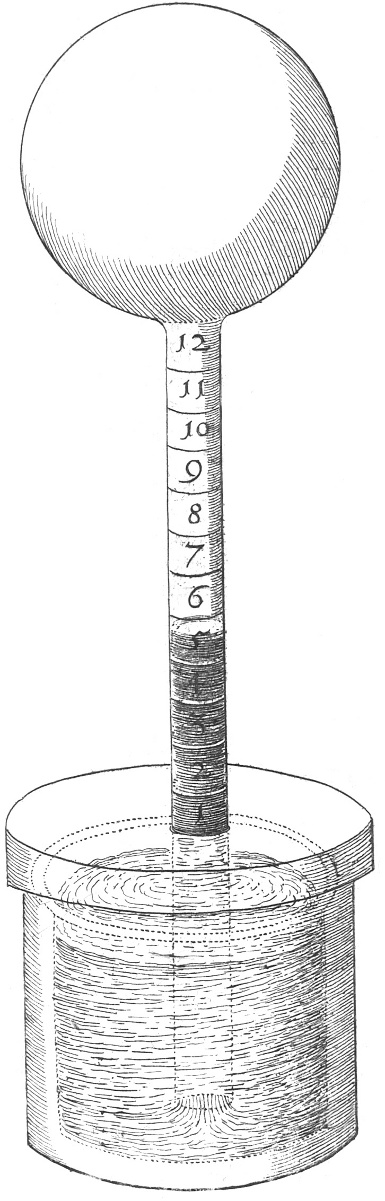
\includegraphics[height=10cm]{images/thermometre_air_1626.jpg}
	\end{center}
	\captionsetup{singlelinecheck=off}
   \captionof{figure}[ding-dong]{Thermomètre à air du début du \textsc{xvii}\ieme siècle. La boule est emplie de gaz dont le volume varie avec sa température, repoussant l’eau du réservoir en dessous dont la surface est à pression atmosphérique. Le liquide peut être coloré, et ses variations de hauteur sont mesurées au moyen d’une graduation. La pression atmosphérique variant avec les conditions météorologiques, elle affecte les mesures : c’est, en quelque sorte, un baro-thermomètre.\begin{credits}Gravure par Robert Fludd (1626, \pd), sélectionnée par Lamouline 2005~\cite{lamouline2005}\end{credits}}
\end{minipage}\hspace{1cm}%
\begin{minipage}[b]{0.45\linewidth}
	\begin{center}
		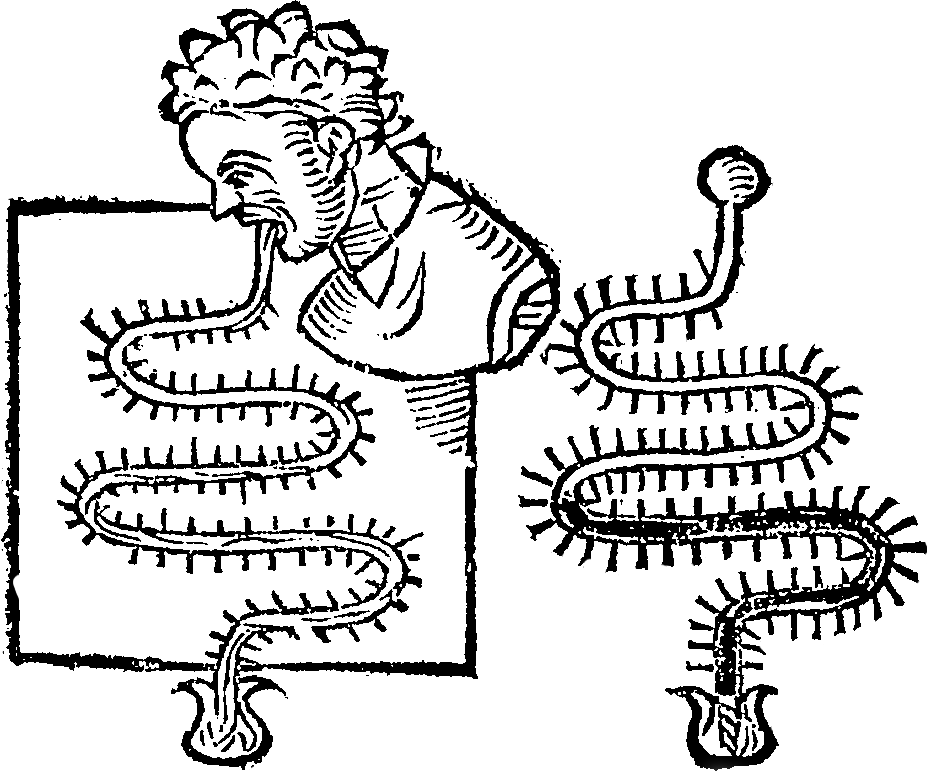
\includegraphics[width=0.9\textwidth]{images/thermometre_medical_1625.png}
	\end{center}
	\captionsetup{singlelinecheck=off}
   \captionof{figure}[ding-dong]{Thermomètre médical du début du \textsc{xvii}\ieme siècle. La boule de gaz était mise en bouche par le patient. On se doute que la sensibilité du thermomètre à la pression atmosphérique n’était pas le plus gros obstacle à son adoption…\begin{credits}Dessin par Santori \& Avicenne (\textit{Commentaria in primam Fen primi libri Canonis Avicennae}, 1625, \pd), sélectionné par Lamouline 2005~\cite{lamouline2005}\end{credits}}
\end{minipage}
\end{landscape}
}%fin onlyframabook

\onlyamphibook{%handmade aaaaannnnnd... this is how it’s done:
	\begin{figure}
		\begin{center}
			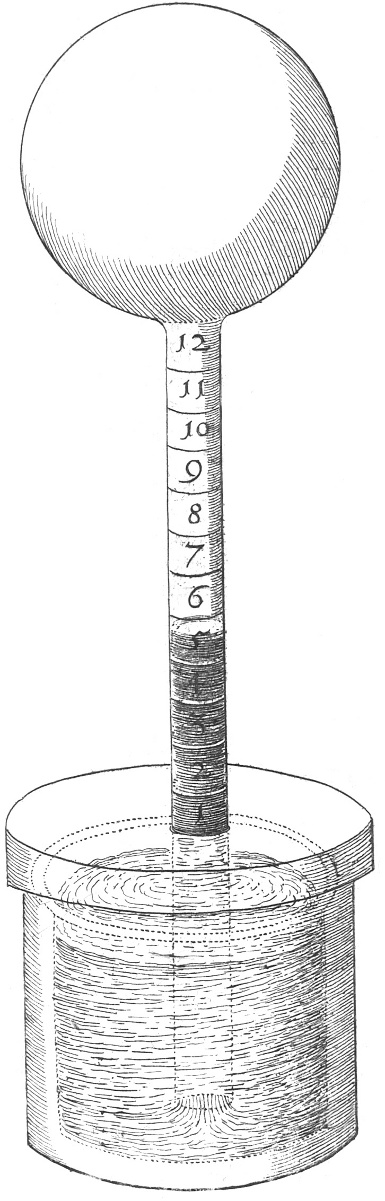
\includegraphics[height=0.6\textwidth]{images/thermometre_air_1626.jpg}
		\end{center}
		\supercaption{Thermomètre à air du début du \textsc{xvii}\ieme siècle. La boule est emplie de gaz dont le volume varie avec sa température, repoussant l’eau du réservoir en dessous dont la surface est à pression atmosphérique. Le liquide peut être coloré, et ses variations de hauteur sont mesurées au moyen d’une graduation. La pression atmosphérique variant avec les conditions météorologiques, elle affecte les mesures : c’est, en quelque sorte, un baro-thermomètre.}{Gravure par Robert Fludd (1626, \pd), sélectionnée par Lamouline 2005~\cite{lamouline2005}}
		\label{fig_thermometre_air}
	\end{figure}
	
	\begin{figure}
		\begin{center}
			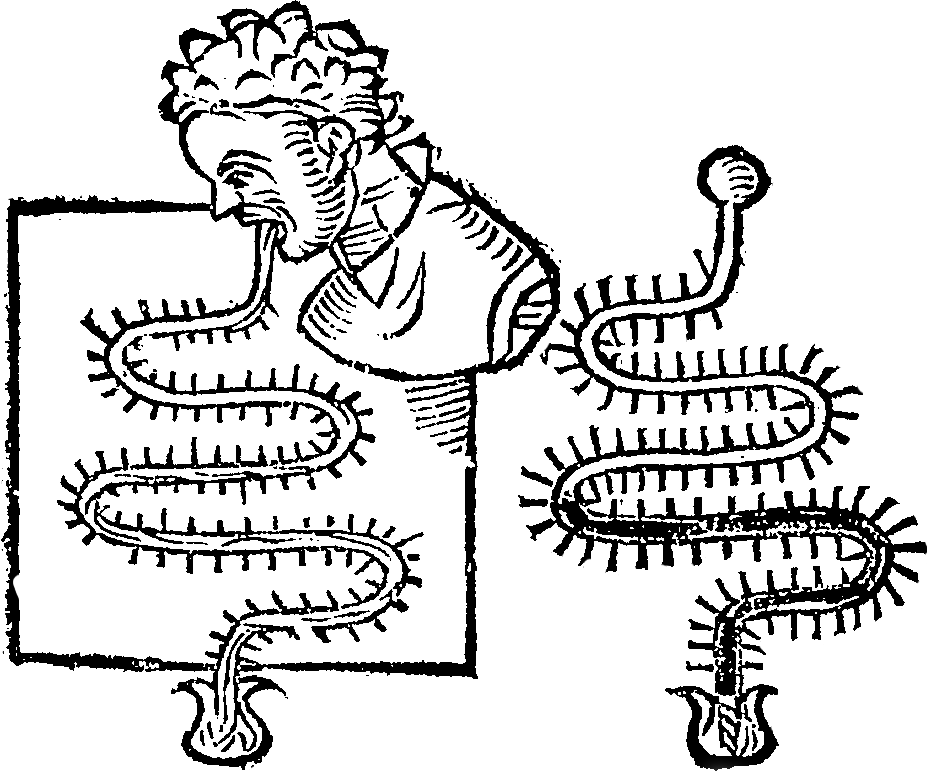
\includegraphics[width=0.5\textwidth]{images/thermometre_medical_1625.png}
		\end{center}
		\supercaption{Thermomètre médical du début du \textsc{xvii}\ieme siècle. La boule de gaz était mise en bouche par le patient. On se doute que la sensibilité du thermomètre à la pression atmosphérique n’était pas le plus gros obstacle à son adoption…}{Dessin par Santori \& Avicenne (\textit{Commentaria in primam Fen primi libri Canonis Avicennae}, 1625, \pd), sélectionné par Lamouline 2005~\cite{lamouline2005}}
		\label{fig_thermometre_medical}
	\end{figure}
	Vers le milieu du siècle, les thermomètres à liquide s'avérèrent beaucoup plus fiables et aussi plus faciles d'emploi. La sphère de verre se trouvait désormais placée en bas du dispositif et était remplie d'un liquide coloré qui montait dans un tube gradué ; ce tube était d'abord ouvert, puis il apparut qu'en le fermant, on évitait l'évaporation du liquide (\cref{fig_thermometre_florence}). Ces perfectionnements avaient été fortement soutenus par le grand-duc italien Ferdinand II de Médicis et ces dispositifs furent ainsi appelés «~thermomètres de Florence~».

	\begin{figure}
		\begin{center}
			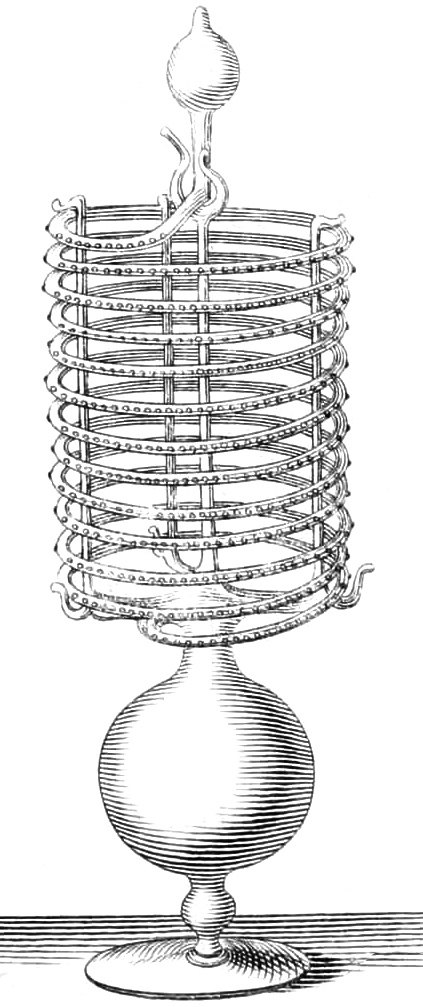
\includegraphics[height=0.7\textwidth]{images/thermometre_florence_1667.jpg}
		\end{center}
		\supercaption{Thermomètre de Florence du milieu du \textsc{xvii}\ieme siècle. Cette fois, c’est le liquide, contenu dans la boule inférieure, qui se contracte et se détend avec la température. Ses variations de volume sont telles qu’un long tube de verre soufflé en spirale est nécessaire pour les mesurer.}{Gravure par l’\textit{Accademia del cimento} (\textit{Staggi di naturali esperientze}, 1667, \pd), sélectionnée par Lamouline 2005~\cite{lamouline2005}}
		\label{fig_thermometre_florence}
	\end{figure}
}%fin onlyamphibook
	
	Restait le problème des graduations. Le nombre de graduations était assez variable, les artisans se bornant à tenter de reproduire ce qu'ils avaient eux-mêmes déjà fait : dans le meilleur des cas des thermomètres construits par la même personne indiquaient à peu près le même résultat. Faute d'échelle universellement acceptée, il était impossible de réaliser des mesures en divers lieux avec des appareils différents pour les comparer.\\
	Dans les premières années du \textsc{xviii}\ieme siècle, le français \wf{Guillaume Amontons} construit un thermomètre à air basé sur la mesure d'une différence de pression et non de volume. Ayant observé que si l'on continuait à chauffer de l'eau bouillante, son degré de chaleur n'augmentait pas, il utilise cette référence comme point fixe. Il fallait évidemment corriger les mesures par une mesure simultanée de la pression atmosphérique. Ce système permet à Amontons de faire une découverte majeure : si la pression du gaz augmente quand le degré de chaleur augmente, à l'inverse, elle diminue quand le degré de chaleur diminue. Au minimum, cette pression doit devenir nulle, ainsi que le degré de chaleur. Ce minimum ainsi extrapolé correspond, en unités modernes, à~\SI{-239,5}{\degreeCelsius}… Une première mesure du zéro absolu !
	
	Tous ces thermomètres restent toutefois d'un emploi délicat qui limite considérablement leur diffusion. \wf{René-Antoine Ferchault de Réaumur}, vers le milieu du \textsc{xviii}\ieme siècle, met au point un thermomètre à mélange eau-alcool dans lequel le degré d'alcool est précisément fixé afin d'assurer la reproductibilité de l'instrument. Il le gradue en choisissant deux références (la glace fondante et l'eau bouillante) et divise cet intervalle en 80 degrés. Cette échelle est appelée «~échelle de Réaumur~».\\	
	En 1724, à Dantzig, l’allemand \wf{Daniel Gabriel Fahrenheit} décrit un thermomètre qui utilise la dilatation du mercure et introduit une échelle pour laquelle la glace fondante est à~\SI{32}{\degree} et la température du sang à~\SI{96}{\degree} ; un mélange de glace, d'eau et de sel d'ammoniac lui donne le zéro de son échelle (\S\ref{thermometres_celsius_fahrenheit}).\\	
	En 1741, le suédois \wf{Anders Celsius} reprend l'échelle de Réaumur mais la divise en 100 intervalles au lieu de 80. Cette convention est assez largement diffusée en France et en 1794, au moment de l'adoption du système métrique par la Convention, c'est l'échelle de Celsius qui est adoptée comme échelle officielle.

	Le passage de la sensation subjective de chaud et de froid à la mesure objective de la température avec des instruments fiables et une échelle universelle, entraîna un grand nombre de constatations qui n'allaient jusqu'alors pas de soi : la température d'une cave n'est pas plus élevée en hiver qu'en été, le fer n'est pas «~plus froid~» que le bois, etc., et, somme toute, tout cela est assez récent !

\atendofhistorysection
